\documentclass[journal,12pt,twocolumn]{IEEEtran}

\usepackage{setspace}
\usepackage{gensymb}

\singlespacing


\usepackage[cmex10]{amsmath}

\usepackage{amsthm}

\usepackage{mathrsfs}
\usepackage{txfonts}
\usepackage{stfloats}
\usepackage{bm}
\usepackage{cite}
\usepackage{cases}
\usepackage{subfig}

\usepackage{longtable}
\usepackage{multirow}

\usepackage{enumitem}
\usepackage{mathtools}
\usepackage{steinmetz}
\usepackage{tikz}
\usepackage{circuitikz}
\usepackage{verbatim}
\usepackage{tfrupee}
\usepackage[breaklinks=true]{hyperref}
\usepackage{graphicx}
\usepackage{tkz-euclide}
\usepackage{float}

\usetikzlibrary{calc,math}
\usepackage{listings}
\usepackage{color} %%
\usepackage{array} %%
\usepackage{longtable} %%
\usepackage{calc} %%
\usepackage{multirow} %%
\usepackage{hhline} %%
\usepackage{ifthen} %%
\usepackage{lscape}
\usepackage{multicol}
\usepackage{chngcntr}

\DeclareMathOperator*{\Res}{Res}

\renewcommand\thesection{\arabic{section}}
\renewcommand\thesubsection{\thesection.\arabic{subsection}}
\renewcommand\thesubsubsection{\thesubsection.\arabic{subsubsection}}

\renewcommand\thesectiondis{\arabic{section}}
\renewcommand\thesubsectiondis{\thesectiondis.\arabic{subsection}}
\renewcommand\thesubsubsectiondis{\thesubsectiondis.\arabic{subsubsection}}


\hyphenation{op-tical net-works semi-conduc-tor}
\def\inputGnumericTable{} %%

\lstset{
%language=C,
frame=single,
breaklines=true,
columns=fullflexible
}
\begin{document}


\newtheorem{theorem}{Theorem}[section]
\newtheorem{problem}{Problem}
\newtheorem{proposition}{Proposition}[section]
\newtheorem{lemma}{Lemma}[section]
\newtheorem{corollary}[theorem]{Corollary}
\newtheorem{example}{Example}[section]
\newtheorem{definition}[problem]{Definition}

\newcommand{\BEQA}{\begin{eqnarray}}
\newcommand{\EEQA}{\end{eqnarray}}
\newcommand{\define}{\stackrel{\triangle}{=}}
\bibliographystyle{IEEEtran}
\providecommand{\mbf}{\mathbf}
\providecommand{\pr}[1]{\ensuremath{\Pr\left(#1\right)}}
\providecommand{\qfunc}[1]{\ensuremath{Q\left(#1\right)}}
\providecommand{\sbrak}[1]{\ensuremath{{}\left[#1\right]}}
\providecommand{\lsbrak}[1]{\ensuremath{{}\left[#1\right.}}
\providecommand{\rsbrak}[1]{\ensuremath{{}\left.#1\right]}}
\providecommand{\brak}[1]{\ensuremath{\left(#1\right)}}
\providecommand{\lbrak}[1]{\ensuremath{\left(#1\right.}}
\providecommand{\rbrak}[1]{\ensuremath{\left.#1\right)}}
\providecommand{\cbrak}[1]{\ensuremath{\left\{#1\right\}}}
\providecommand{\lcbrak}[1]{\ensuremath{\left\{#1\right.}}
\providecommand{\rcbrak}[1]{\ensuremath{\left.#1\right\}}}
\theoremstyle{remark}
\newtheorem{rem}{Remark}
\newcommand{\sgn}{\mathop{\mathrm{sgn}}}
\providecommand{\abs}[1]{\left\vert#1\right\vert}
\providecommand{\res}[1]{\Res\displaylimits_{#1}}
\providecommand{\norm}[1]{\left\lVert#1\right\rVert}
%\providecommand{\norm}[1]{\lVert#1\rVert}
\providecommand{\mtx}[1]{\mathbf{#1}}
\providecommand{\mean}[1]{E\left[ #1 \right]}
\providecommand{\fourier}{\overset{\mathcal{F}}{ \rightleftharpoons}}
%\providecommand{\hilbert}{\overset{\mathcal{H}}{ \rightleftharpoons}}
\providecommand{\system}{\overset{\mathcal{H}}{ \longleftrightarrow}}
%\newcommand{\solution}[2]{\textbf{Solution:}{#1}}
\newcommand{\solution}{\noindent \textbf{Solution: }}
\newcommand{\cosec}{\,\text{cosec}\,}
\providecommand{\dec}[2]{\ensuremath{\overset{#1}{\underset{#2}{\gtrless}}}}
\newcommand{\myvec}[1]{\ensuremath{\begin{pmatrix}#1\end{pmatrix}}}
\newcommand{\mydet}[1]{\ensuremath{\begin{vmatrix}#1\end{vmatrix}}}
\numberwithin{equation}{subsection}
\makeatletter
\@addtoreset{figure}{problem}
\makeatother
\let\StandardTheFigure\thefigure
\let\vec\mathbf
\renewcommand{\thefigure}{\theproblem}
\def\putbox#1#2#3{\makebox[0in][l]{\makebox[#1][l]{}\raisebox{\baselineskip}[0in][0in]{\raisebox{#2}[0in][0in]{#3}}}}
\def\rightbox#1{\makebox[0in][r]{#1}}
\def\centbox#1{\makebox[0in]{#1}}
\def\topbox#1{\raisebox{-\baselineskip}[0in][0in]{#1}}
\def\midbox#1{\raisebox{-0.5\baselineskip}[0in][0in]{#1}}
\vspace{3cm}
\title{Assignment No.5}
\author{Valli Devi Bolla}
\maketitle
\newpage
\bigskip
\renewcommand{\thefigure}{\theenumi}
\renewcommand{\thetable}{\theenumi}
Download all python codes from
\begin{lstlisting}
https://github.com/Vallidevibolla/Assignment-5/blob/main/code.py
\end{lstlisting}
%
and latex-tikz codes from
%
\begin{lstlisting}
https://github.com/Vallidevibolla/Assignment-5/blob/main/main.tex
\end{lstlisting}
%
Question taken from
\begin{lstlisting}
https://github.com/gadepall/ncert/blob/main/linalg/quadratic_forms/gvv_ncert_quadratic_forms.pdf-Q.no.2.7
\end{lstlisting}
%
%https://github.com/gadepall/ncert/blob/main/linalg/linman/chapters/conics/tangent_normal.tex
%
\section{Question 2.7}
Find the area of the region bounded by curve 
%\cite{twelve_one}
\begin{align}
\vec{y^2} = \vec{x}
\label{eq:parab}
\end{align}
and the lines \vec{x}=1,\vec{x}=4 and x-axis in the first quadrant.
\\
\section{Solution}
\eqref{eq:parab} can be written as
\begin{align}
y^2 - x &= 0
\label{eq:parab_twovar}
\end{align}

The matrix parameters  are
\begin{align}
\vec{V} = \myvec{0 & 0\\0 & 1}, \vec{u} = \myvec{\frac{-1}{2}\\0}, \vec{f}=0.
\label{eq:parab_twovar_params}
\end{align}
Thus, the given curve is a parabola.  $\because \vec{V}$ is diagonal and in standard form,
Also, 
\begin{align}
\vec{V}\vec{p} &= \vec{0}
\\
\implies \vec{p} &= \myvec{1\\0}
\label{eq:parab_twovar_p}
\end{align}
with eigen parameters\\
\begin{align}
\lambda_1=0, \lambda_2=1
\end{align}
Given \vec{x}=1  Using \eqref{eq:parab} we get
\begin{align}
\vec{x}=\myvec{1\\0}+\vec{y}\myvec{0\\1}\\
\myvec{1 & 0}\vec{x}=\myvec{1 & 0}\myvec{1\\0}+\vec{y}\myvec{1 & 0}\myvec{0\\1}\\
\myvec{1 & 0}\vec{x}=1\label{eq:line1}
\end{align}
Similarly, \vec{x}=4 we get
\begin{align}\label{eq:line2}
\myvec{4 & 0}\vec{x}=16\\
\implies\myvec{1 & 0}\vec{x}=4
\end{align}
The direction vector and normal vectors are
\begin{align}
\vec{m} = \myvec{0\\1}, \vec{n} = \myvec{1\\0}.
\label{eq:parab_twovar_mn}
\end{align}
The equation of parabola is
\begin{align}
\vec{q}^T\vec{V}\vec{q} + 2\vec{u}^T\vec{q} +f = 0
\label{eq:conic_tangent_qquad}
\end{align}\\
The vertex of conic section in \eqref{eq:conic_tangent_qquad} is given by \vec{c} using  
\begin{align}
\label{eq:vertex}
\begin{pmatrix}
\vec{u^T+n \vec{p}}^T \\ \vec{V}
\end{pmatrix}
\vec{c} &= 
\begin{pmatrix}
-f
\\
\vec{n}\vec{p}-\vec{u}
\end{pmatrix}
\end{align}
\begin{align}
\myvec{\frac{1}{2} & 0 \\ 0 & 0 \\ 0 & 1}\vec{c} &= \myvec{0 \\ 0\\\frac{3}{2}} 
\\
\implies 
\myvec{\frac{1}{2} & 0 \\  0 & 1}\vec{c} &= \myvec{0 \\ \frac{3}{2}} 
\\
\text{or, } \vec{c} = \myvec{0\\\frac{3}{2}}
\end{align}
\begin{align}
\label{eq:conic_tangent_qk_eigen} \kappa = \frac{\vec{p}_1^T\vec{u}}{\vec{p}_1^T\vec{n}}, \quad 
\end{align}
From \eqref{eq:conic_tangent_qk_eigen}, \eqref{eq:parab_twovar_mn} and \eqref{eq:parab_twovar_p},
\begin{align}
\kappa = 0
\end{align}
which, upon substitution in  \eqref{eq:conic_tangent_q_eigen}
\begin{align}
\label{eq:conic_tangent_q_eigen}
\begin{pmatrix}
\vec{u+\kappa \vec{n}}^T \\ \vec{V}
\end{pmatrix}
\vec{q} &= 
\begin{pmatrix}
-f
\\
\kappa\vec{n}-\vec{u}
\end{pmatrix}
\end{align}
and simplification yields the matrix equation
\begin{align}
\myvec{\frac{-1}{2} & 0 \\0 & 0\\0&1}\vec{q} &= \myvec{0\\0\\\frac{1}{2}}
\\
\implies \myvec{\frac{-1}{2} & 0\\0&1}\vec{q} &= \myvec{0\\\frac{1}{2}}
\\
\text{or, } \vec{q} &= \myvec{0 \\\frac{1}{2}}
\end{align}
\item 
{\em Secant: }The points of intersection of the line 
\begin{align}
L: \quad \vec{x} = \vec{q} + \mu \vec{m} \quad \mu \in \mathbb{R}
\label{eq:conic_tangent}
\end{align}
\begin{align}\label{eq:parametricform}
\vec{x}_i = \vec{q} + \mu_i \vec{m}
\end{align}
%
where
\begin{multline}
\mu_i = \frac{1}
{
\vec{m}^T\vec{V}\vec{m}
}
\lbrak{-\vec{m}^T\brak{\vec{V}\vec{q}+\vec{u}}}
\\
\pm
{\small
\rbrak{\sqrt{
\sbrak{
\vec{m}^T\brak{\vec{V}\vec{q}+\vec{u}}
}^2
-
\brak
{
\vec{q}^T\vec{V}\vec{q} + 2\vec{u}^T\vec{q} +f
}
\brak{\vec{m}^T\vec{V}\vec{m}}
}
}
}
\label{eq:tangent_roots}
\end{multline}
                    
$\because \vec{q}$ is the point of contact, $\vec{q}$ satisfies parabola equation

\item 
Given the point of contact $\vec{q}$, the equation of a tangent is 
\begin{align}
\brak{\vec{V}\vec{q}+\vec{u}}^T\vec{x}+\vec{u}^T\vec{q}+f = 0
\label{eq:conic_tangent_final}
\end{align}

From \eqref{eq:tangent_roots} we get \\
\mu_=\frac{-1}{2}

The lines \eqref{eq:line1}, \eqref{eq:line2} can be written in parametric form in \eqref{eq:parametricform} we get\\
\begin{align}\label{eq:para1}
\vec{x}_i = \myvec{\frac{3}{4}\\ \frac{1}{2}} + \mu_i \myvec{0\\1}
\end{align}
Substituting \mu value in \eqref{eq:para1} we get

\begin{align}
\vec{x}_i_1 = \myvec{0\\ \frac{1}{2}} + \frac{-1}{2}\myvec{0\\1}\\
\implies\vec{K}=\myvec{0\\0}
\end{align}
The area enclosed by parabola and line can be given as\\
A = Area under line - Area under curve
\begin{align}
\implies\boxed{\vec{A} = \vec{A_1}-\vec{A_3}} \label{eq:A}
\end{align}
Thus area under the lines \eqref{eq:line1} , \eqref{eq:line2} is given by

\vec{A_1} =\frac{1}{2},
\vec{A_2}=\frac{-17}{2}   
  
Area under the parabola\eqref{eq:parab} i.e,

\vec{A_3} =$\int$\vec{x}^\frac{1}{2} dx \\
\implies\boxed{\vec{A_3} =\frac{14}{3}}

Putting these values in \eqref{eq:A} we get\\
\vec{A} =-4.17,-13.17 units


\numberwithin{figure}{section}
\begin{figure}[!ht]
\centering
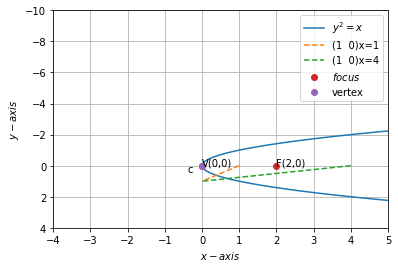
\includegraphics[width=\columnwidth]{download.png}
\caption{Parabola \vec{y^2} = \vec{x} }
\label{fig:parab_tangent}	
\end{figure}

\end{document}
